\documentclass{article}
\usepackage{graphicx} % new way of doing eps files
\usepackage{listings} % nice code layout
\usepackage[usenames]{color} % color
\definecolor{listinggray}{gray}{0.9}
\definecolor{graphgray}{gray}{0.7}
\definecolor{ans}{rgb}{1,0,0}
\definecolor{blue}{rgb}{0,0,1}
% \Verilog{title}{label}{file}
\graphicspath{ {H:/ELC3338/Team8/CompOrg_Spring2018_S1_Team8/images/} }
\newcommand{\Verilog}[3]{
  \lstset{language=Verilog}
  \lstset{backgroundcolor=\color{listinggray},rulecolor=\color{blue}}
  \lstset{linewidth=\textwidth}
  \lstset{commentstyle=\textit, stringstyle=\upshape,showspaces=false}
  \lstset{frame=tb}
  \lstinputlisting[caption={#1},label={#2}]{#3}
}


\author{Matthew Carrano and Breana Leal}
\title{Lab 4: Beginning to Decode}

\begin{document}
\maketitle

\section{Simplified Report}
The instr\_parse module uses both R and D format to break down instruction code. The module parses the instruction bits successfully and it is verified using four the instruction codes provided in class.
The regfile module reads data from the regData file into an array of registers. The module releases the addressed data into the register array using non-blocking assignments and outputs the instruction into read\_data1 and read\_data2, based on the read\_reg indices. When write\_data input is HIGH, data will be written to a register in the array specified by the write\_reg index. This action is verified through the simulation. 

\section{Code}
\Verilog{Verilog code for implementing the instr\_parse module.}{code:adder}{../code/decode/instr_parse.v}



\Verilog{Verilog code for implementing the regfile module.}{code:mux}{../code/decode/regfile.v}


\section{Testbench}

\Verilog{Verilog code for implementing the instr\_parse testbench.}{code:adder}{../code/decode/instr_parse_test.v}


\Verilog{Verilog code for implementing the regfile testbench.}{code:mux}{../code/decode/regfile_test.v}




\section{Simulation}
As seen from the simulation in Figure 2, the read\_data output registers equal the addresses given in the read\_reg inputs. This is simply because we altered the regData file to the values show in Figure 3.

\begin{figure}[h]	
	\caption{Timing diagram for instr\_parse module test.}
	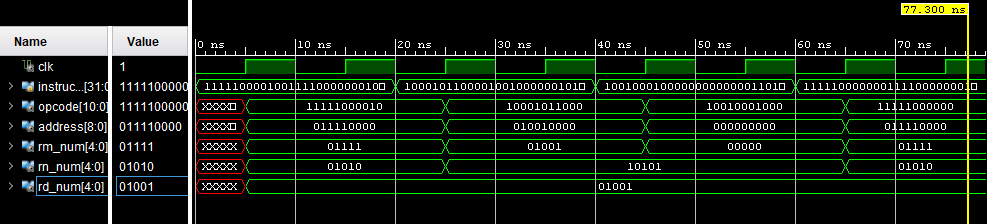
\includegraphics[width=\textwidth]{instr_parse_sim}
	
\end{figure}

\begin{figure}[h]	
	\caption{Timing diagram for regfile module test.}
	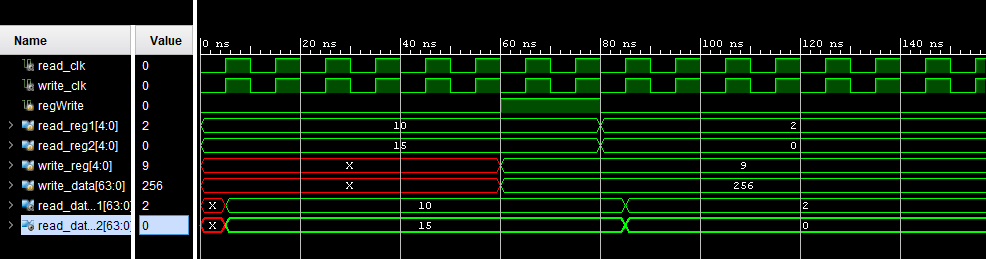
\includegraphics[width=\textwidth]{regfile_sim}
	\label{fig:fetchtest}
\end{figure}
\begin{figure}[h]	
	\caption{Modified Register File Data.}
	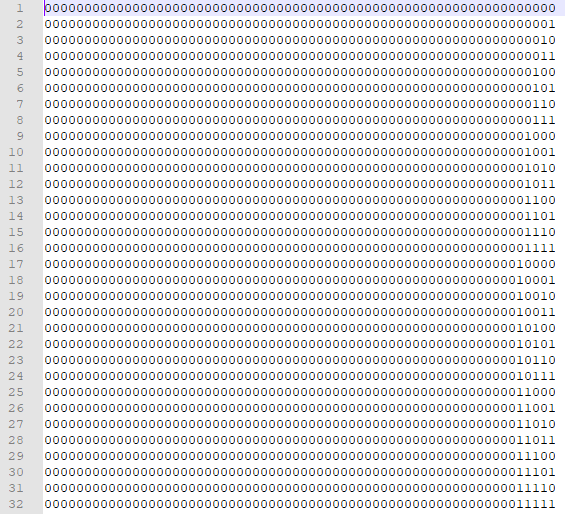
\includegraphics[width=\textwidth]{Modified_data}
	\label{fig:fetchtest}
\end{figure}
 
\end{document} 